\documentclass[a4paper,11pt,oneside]{book}
\usepackage{latexsym}
\usepackage{braket}
\usepackage{graphicx}
\usepackage{amsfonts}
\usepackage{amsmath}
\usepackage{verbatim}
\usepackage{amssymb}
\usepackage{amsthm}
\usepackage{graphicx}
\usepackage[english]{babel}
\usepackage[utf8]{inputenc}
\usepackage{listings}
\usepackage{color}
\usepackage{float}


\pagestyle{plain}

\lstset{
  basicstyle=\ttfamily,
  columns=fullflexible,
  showstringspaces=false,
  commentstyle=\color{gray}\upshape
}

\lstset{ 
  breakatwhitespace=false,         % sets if automatic breaks should only happen at whitespace
  breaklines=true,                 % sets automatic line breaking
  captionpos=b,                    % sets the caption-position to bottom
  frame=single,                    % adds a frame around the code
  keepspaces=true,                 
  numbers=left,                    % where to put the line-numbers; possible values are (none, left, right)
  numbersep=5pt,                   % how far the line-numbers are from the code
  numberstyle=\tiny\color{gray}, % the style that is used for the line-numbers
  rulecolor=\color{black},         % if not set, the frame-color may be changed on line-breaks within not-black text (e.g. comments (green here))
  showtabs=false,                  % show tabs within strings adding particular underscores
  stepnumber=1,                    % the step between two line-numbers. If it's 1, each line will be numbered
  tabsize=2,                       % sets default tabsize to 2 spaces
  title=\lstname,                   % show the filename of files included with \lstinputlisting; also try caption instead of title
 language=C++,
 %basicstyle=\footnotesize,        % the size of the fonts that are used for the code
 basicstyle=\ttfamily,
 morekeywords={A}, 
 keywordstyle=\color{darkblue}\ttfamily,
 %identifierstyle=\color{green},
 stringstyle=\color{red}\ttfamily,
 %numberstyle=\color{purple}
 commentstyle=\color{gray}\ttfamily,
 morecomment=[l][\color{red}]{\#}
}

\definecolor{darkblue}{rgb}{0.0,0.0,0.8}
\definecolor{green}{rgb}{0,0.6,0}
\definecolor{gray}{rgb}{0.5,0.5,0.5}
\definecolor{darkgray}{rgb}{0.105,0.105,0.105}
\definecolor{mauve}{rgb}{0.58,0,0.82}
\definecolor{black}{rgb}{0,0,0}
\definecolor{purple}{rgb}{0.72,0.61,0.139}
%\definecolor{ocra}{rgb}{0.204, 0.119, 0.34}
\definecolor{ocra}{rgb}{0.184,0.134,0.11}
\definecolor{maroon}{rgb}{0.5,0,0}
\definecolor{darkgreen}{rgb}{0,0.5,0}
\lstdefinelanguage{XML}
{
  basicstyle=\ttfamily,
  morestring=[s]{"}{"},
  morecomment=[s]{?}{?},
  morecomment=[s]{!--}{--},
  commentstyle=\color{darkgreen},
  moredelim=[s][\color{black}]{>}{<},
  moredelim=[s][\color{red}]{\ }{=},
  stringstyle=\color{blue},
  identifierstyle=\color{maroon}
}


\author{Giacomo Dabisias, Filippo Brizzi}
\title{A framework for static allocation of parallel OpenMp code on multi-core platforms}
\frenchspacing

\begin{document}
\frontmatter
\tableofcontents

\chapter{Abstract}

The aim of this thesis is to create a framework for guaranteeing \emph{real-time} constraints on parallel \emph{OpenMP} C++ code. The framework provides a static schedule for the allocation of tasks on system threads and a run-time support for the \emph{real-time} execution. In order to do so the original source code is first instrumented, then profiled and finally rewritten by means of clang. Performance results are provided on a Computer Vision application.

\section{Chapter's structure}

\mainmatter
\chapter{Introduction}

\section{Motivation, context and target application}

The last years have seen the transition from single core architectures towards multicore architectures, mainly in the desktop and server enviroment. Lately also small devices as smartphones, embedded microprocessors and tablets have started to use more than a single core processor. The actual trend is to use a lot of cores with just a reduced instruction set as in \emph{general purpose GPUs}.

Also \emph{real time} systems are becoming more and more common, finding their place in almost all aspects of our daily routines; this systems often consist of several applications executing concurrently on shared resources. 
The main differences between this systems and a system designed to achive high performance can be summarized as follows:
\begin{itemize}
\item{ \emph{Real time} programs need strict timing guarantees, while high performance programs try to achive the lowest possible computation time, usually in a best effort manner.}
\item{\emph{Real time} programs need to be predictable; in principle it could be that a real time program could finish almost always before its deadline on a high performance system, but it could be that in some exceptional cases, due to execution preemption, context switches, concurrent resource access \dots the program does not finish in time. To solve this, it may happen that the mean execution time of the real time program grows, but the program becomes also predictable, in the sense that it always finishes within its deadline.}
\item{ High performance systems need to "scale" well when the architecture becomes more powerful, while \emph{real time} systems need just to satisfy the timing contrains, even with no performance gain.}

\end{itemize}

The most relevant drawback of actual real time systems is that most of them are usually made to exploit just one single computing core, while their capabilities demand is growing. Applications like Computer Vision, Robotics, Simulation, Video Encoding/Decoding, Software Defined Radios,\dots have the necessity to process in parallel more tasks to achive a positive feedback for the user. This bring to two possible solutions:
\begin{itemize}
\item{Find new and better scheduling algorithms to allocate new tasks using the same single core architecture}
\item{Upgrade the processing power by adding new computing cores or by using a faster single core.}
\end{itemize}

The first solution has the disadvantage that, if the computing resources are already perfectly allocated, it is not possible to find any better scheduling for the tasks to make space for a new job. A faster single core is also often not feasible, given the higher power consumption and temperature; this aspect is very relevant in embedded devices. 
The natural solution to the problem is to exploit the new trend toward multicore systems; this solution has opened a new research field and has brought to view a lot of new challenging problems. Given that the number of cores is doubling according to the well known \emph{Moores law}, it is very important to find a fast and architecture independent way to map a set of \emph{real time} tasks on computing cores. With such a tool, it would be possible to upgrade or change the computing architecture in case of new \emph{real time} jobs, just scheduling them on the new system.


\section{Objective}

To overcome the problems stated before, the described tool must have four fundamental features:
\begin{itemize}
\item{An easy \emph{API} for the programmer to specify the concurrency between \emph{real time} tasks together with all the necessary scheduling parameters (deadlines, computation times, activation times \dots)}
\item{A way to visualize task concurrency and code structure as graphs.}
\item{A \emph{scheduling algorithm} which supports multicore architectures, adapting to the specific platform.}
\item{A \emph{run time support} for the program execution which guarantees the scheduling order of tasks and their timing contrains.}
\end{itemize}


\section{Supporting parallelism in C/C++}
\section{The OpenMP standard}

Jointly defined by a group of major computer hardware and software vendors, \emph{OpenMP} is a portable, scalable model that gives shared-memory parallel programmers a simple and flexible interface for developing parallel applications for platforms ranging from desktop to the supercomputer.

The \emph{OpenMP API} uses the fork-join model of parallel execution. Multiple threads of execution perform tasks defined implicitly or explicitly by \emph{OpenMP} directives. The \emph{OpenMP API} is intended to support programs that will execute correctly both as parallel programs (multiple threads of execution and a full \emph{OpenMP} support library) and as sequential programs (directives ignored and a simple \emph{OpenMP} stubs library).
An \emph{OpenMP} program begins as a single thread of execution, called an initial thread. An initial thread executes sequentially, as if enclosed in an implicit task region, called an initial task region, that is defined by the implicit parallel region surrounding the whole program.

If a construct creates a data environment after an \emph{OpenMP} directive, the data environment is created at the time the construct is encountered. Whether a construct creates a data environment is defined in the description of the construct. When any thread encounters a parallel construct, the thread creates a team of itself and zero or more additional threads and becomes the master of the new team. The code for each task is defined by the code inside the parallel construct. Each task is assigned to a different thread in the team and becomes tied; that is, it is always executed by the thread to which it is initially assigned. The task region of the task being executed by the encountering thread is suspended, and each member of the new team executes its implicit task. Each directive uses a number of threads defined by the standard or it can be set using the function call \emph{void omp\_set\_num\_threads(int num\_threads)}. In this project this call is not allowed and the thread number for each directive is managed separately. There is an implicit barrier at the end of each parallel construct; only the master thread resumes execution beyond the end of the parallel construct, resuming the task region that was suspended upon encountering the parallel construct. Any number of parallel constructs can be specified in a single program. 

It is very important to notice that \emph{OpenMP}-compliant implementations are not required to check for data dependencies, data conflicts, race conditions, or deadlocks, any of which may occur in conforming programs. In addition, compliant implementations are not required to check for code sequences that cause a program to be classified as non conforming. Also the developed tool will only accept well written programs, whitout checking if they are \emph{OpenMP}-compliant. The \emph{OpenMP} specification makes also no guarantee that input or output to the same file is synchronous when executed in parallel. In this case, the programmer is responsible for synchronizing input and output statements (or routines) using the provided synchronization constructs or library routines; this assumption is also maintained in the developed tool.

In C/C++, \emph{OpenMP} directives are specified by using the\begin{bf} $\#$pragma\end{bf} mechanism provided by the C and C++ standards.  Almost all directives start starts with \begin{bf}$\#$pragma omp\end{bf} and have the following grammar:
\begin{bf}{\center{$\#$pragma omp directive-name [clause[ [,] clause]...] new-line}}\end{bf}
\\

A directive applies to at most one succeeding statement, which must be a structured block, and may be composed of consecutive $\#$pragma preprocessing directives. 

It is possible to specify for each variable, in an \emph{OpenMP} directive, if it should be private or shared by the threads; this can be done using the clause attribute \emph{shared(variable)} or \emph{private(variable)}\\
There is a big variety of directives which permit to express almost all computational patterns; for this reason a restricted set has been choosen in this project. Real time applications tend to be composed by a lot of small jobs, with only a small amount of shared variables and a lot of controllers. Given this, the following \emph{OpenMP} directives have been choosen:
\begin{itemize}
\item{\begin{bf}{$\#$pragma omp parallel}\end{bf} : all the code inside of this block is executed in parallel by all the available threads. Each thread has its variables scope defined by the appropriate clauses. }
\item{\begin{bf}{$\#$pragma omp sections}\end{bf} : this pragma opens a block which has to contain section directives; it has always to be contained inside a \begin{bf}$\#$pragma omp parallel block\end{bf}. There is an implicit barrier at the end of this block synchronizing all the section blocks which are included. }
\item{\begin{bf}{$\#$pragma omp section}\end{bf} : all the code inside of this block is executed in parallel by only \emph{one} thread. }
\item{\begin{bf}{$\#$pragma omp for}\end{bf} : this pragma must precede a for cycle. In this case the \emph{for loop} is splitted among  threads and a private copy of the looping variable is associated to each. This pragma must be nested in a \begin{bf}$\#$pragma omp parallel\end{bf} directive or can be expressed as \begin{bf}{$\#$pragma omp parallel for}\end{bf} without the need of the previous one.  }
\item{\begin{bf}{$\#$pragma single}\end{bf} : this pragma must be nested inside a \begin{bf}{$\#$pragma omp parallel }\end{bf} and means that the code block contained in it must be executed only by a single thread}
\item{\begin{bf}{$\#$pragma task}\end{bf} : this pragma must be nested inside a \begin{bf}{$\#$pragma omp parallel }\end{bf} and means that all the possible threads will execute in parallel the same code block contained in it. In the developed tool this structure is not allowed. The allowed structure instead is composed by a number of \begin{bf}{$\#$pragma task}\end{bf} nested inside a \begin{bf}{$\#$pragma single}\end{bf} block. The semantic of this contruct is the same as  having \begin{bf}{$\#$pragma omp section}\end{bf}s inside \begin{bf}{$\#$pragma omp sections}\end{bf}.}
\end{itemize}

The considered pragma set can be splitted into two groups: 
\begin{itemize}
\item{ A first set composed of \begin{bf}{$\#$pragma omp parallel}\end{bf}, \begin{bf}{$\#$pragma omp sections}\end{bf} and \begin{bf}{ $\#$pragma omp single}\end{bf} which are “control” pragmas, meaning that they are used to organize the task execution.}
\item{A second set containing \begin{bf}{$\#$pragma omp section}\end{bf}, \begin{bf}{$\#$pragma omp task}\end{bf} and \begin{bf}{$\#$pragma omp for}\end{bf} which represent “jobs”, since they contain the majority of the computation code.}
\end{itemize}

 \emph{OpenMP} imposes that pragmas belonging to the second group must always be nested inside a control pragma and that no pragmas can be nested inside them. It is still possible to overcome this rule by invoking a function, which contains pragmas, inside one of the pragmas contained in the first group; however to make this approach work it is necessary to set the \emph{OMP\_NESTED} environment variable by invoking the function call \emph{omp\_set\_nested(1)}.

With this subset of \emph{OpenMP} it is possible to create all the standard computation patterns like \emph{Farms}, \emph{Maps}, \emph{Stencils} \dots 

\emph{OpenMp} synchronization directives as \begin{bf}$\#$pragma omp barrier\end{bf} are not supported for now; only the synchronization semantic given by the above directives is ensured. 

\section{Clang as LLVM frontend}

\chapter{Design}
\section{The framework}

The framework takes as input a C++ source code annotated with \emph{OpenMP} and translates each pragma block in a task. After that the tool searches for the best possible schedule that satisfies the tasks timing contrains. The source code is then executed with the given schedule and the help of a newly produced run-time support.

The developed tool works accordingly to the following steps:
\begin{itemize}
\item{the \emph{AST}, Abstract Sintax Tree, of the source code is created using \emph{Clang}. From this all the relevant information of each \emph{OpenMP} pragma are extracted and inserted in a properly formatted \emph{XML} file.}
\item{Each pragma in the source code is substituted with a proper profiling function call. The execution of the new code produces a log file which includes, for each pragma, timing informations.  }
\item{The new source code and the pragma \emph{XML} file are given as imput to a second tool written in \emph{Python}. This tool parses the \emph{XML} file and creates a graph which represents the parallel execution flow of the tasks. After that it executes the given profiled source code $N$ times creating statistics of the execution. The graph, enhanced with the new profiling information, is saved as a new \emph{XML} file}
\item{ A scheduling algorithm is run on the created graph to find the best possible scheduling sequence accordingly to the profiling information. The found scheduling is then checked to be compatible with the precedence contraints given by the \emph{OpenMP} standard and, in case, a \emph{XML} schedule file is created.}
\item{ The source code is rewritten substituting to each pragma a proper code block for the creation of the tasks. During the execution each task is passed to the run-time support which allocates it accordingly to the previously creted schedule.}
\end{itemize}

Picture \ref{framework} gives a visual representation of the framwork.


\begin{figure}[H]
\centering
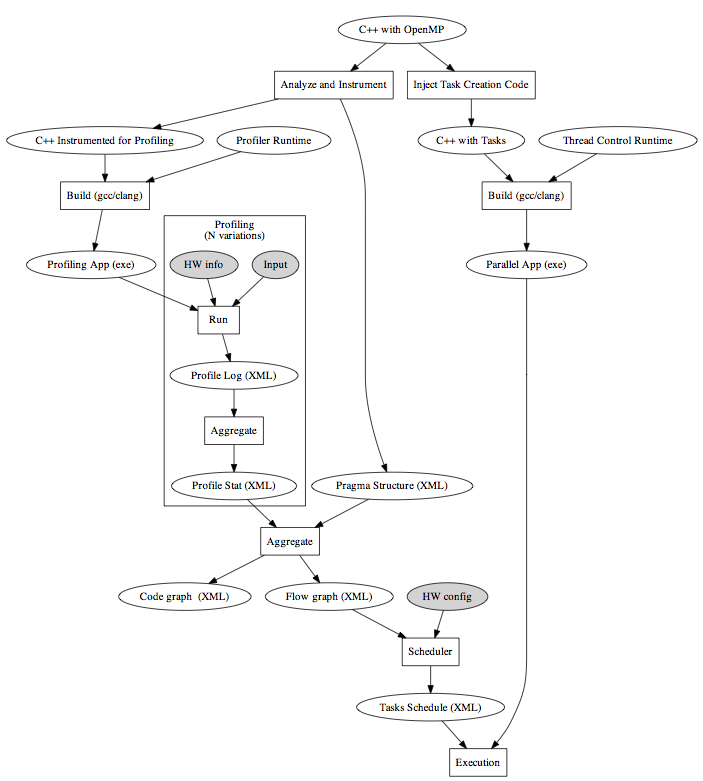
\includegraphics[width = 160mm, height = 180mm]{framework.png}
\caption{The famework structure}
\label{framework}
\end{figure}


\section{A simple example}

A simple example has been developed in order to show how the tool works in each step. Given the \emph{OpenMP} semantic described before, the two \begin{bf}$\#$pragma omp section\end{bf} are executing in parallel abd synchronize at the end of the \begin{bf}$\#$pragma omp parallel private(bar)\end{bf}. The clause \emph{private(bar)} makes the \emph{bar} variable private to each thread in order to have no race condition. To execute the code with some timing constrains some code has been added inside of the for loop which is not relevant for the explaination purpose.

\lstset{language=C++}
\begin{lstlisting}[caption=Sample code, label=code]

#include <omp.h>

int work(int bar){
    #pragma omp parallel for
    for (int i = 0; i < bar; ++i)
    {
       //do stuff
    }  
    return 0;
};

int main(int argc, char* argv[]) {
    int bar;
    #pragma omp parallel private(bar)
    {
        #pragma omp sections
        {
            #pragma omp section
            {   
                //do stuff (bar)
                work(bar);
            }
            
            #pragma omp section
            {
                //do stuff (bar)
                work(bar);
            }
        }
    }
    return 0;
}

\end{lstlisting}


\section{Analysis}
\subsection{Code}
\subsection{Parallelism}

Using the previously created \emph{XML} file, which contains all the pragmas present in the source code, two different graphs are created. The first one reflects the pragmas structure in the source code, while the second one displays the execution flow of the different pragma blocks. Each pragma is represented by a node which contains all the relevant informations. All nodes derive from a general \emph{Node} class; the most relevant attributes are the following:
\begin{itemize}
\item{ptype : represents the type of the pragma.}
\item{start\_line : represents the code line where the pragma block starts.}
\item{children : a list of all the children pragmas.}
\item{parents : a list of all the pragma parents.}
\item{time : the execution time of the pragma.}
\item{variance : the variance of the execution time.}
\item{deadline : the deadline of the task.}
\item{arrival : the arrival time of the task.}
\end{itemize}

Depending on the specific pragma special classes are derived like \emph{For\_Node} in case of a \begin{bf}\emph{$\#$pragma omp for}\end{bf} or \begin{bf}\emph{$\#$pragma omp parallel for}\end{bf} or \emph{Fx\_Node} in case of a function node.

To create the first graph the tool starts parsing the \emph{XML} file and creating a proper object for each encountered pragma. It is important to notice that also pragmas which are not actually executed will be inserted in the graphs. 

The second graph is created taking care of the execution semantic given by \emph{OpenMp}. Again the \emph{XML} file is parsed and an object is created for each pragma. Each object is then connected with the proper ones and if necessary fake \emph{Barrier} nodes are added to guarantee the synchronization given by the standard. This special nodes are added whenever a "control" pragma is encountered; this is due to the fact that this type of pragmas use to have more than one children, creating a sort of diamond topology, which have to synchronize at the end of the pragma block fig:\ref{call_graph}.

\section{Visual graph generation}

To visualize the code structure, parallel code execution and the function call graph, three different type of graphs have been generated, each containing a series of nodes which are connected through undirected archs. The first node of each graph displays the function name along with the total computation time. For each function in the source code a different graph is created in two different formats; for visualization a \emph{PDF} file, while a \emph{DOT} file is created so that the graph can be manipulated with other tools. The code structure graph, simply called code graph, shows how pragmas are nested inside each other. Each node displays relevant informations as pragma type, starting line, execution time and variance. The parallel code execution graph, called flow graph, shows which nodes can be executed in parallel; some simple rules apply in this case to understand the execution flow:
\begin{itemize}
\item{a node can execute only after all the parents have completed.}
\item{All nodes which have a single parent in common can execute in parallel (this is shown by having the same color for arches which can execute in parallel).}
\item{All nodes have to synchronize on barrier nodes.}
\end{itemize}
In the call graph each node invoking a function containing pragmas is connected to the function subgraph by a directed arch fig:\ref{call_graph}; the execution flow continues after the function call terminates and resumes in the children of the caller node. The semantic of the execution is the same as the one of the flow graph.

\begin{figure}[H]
\centering
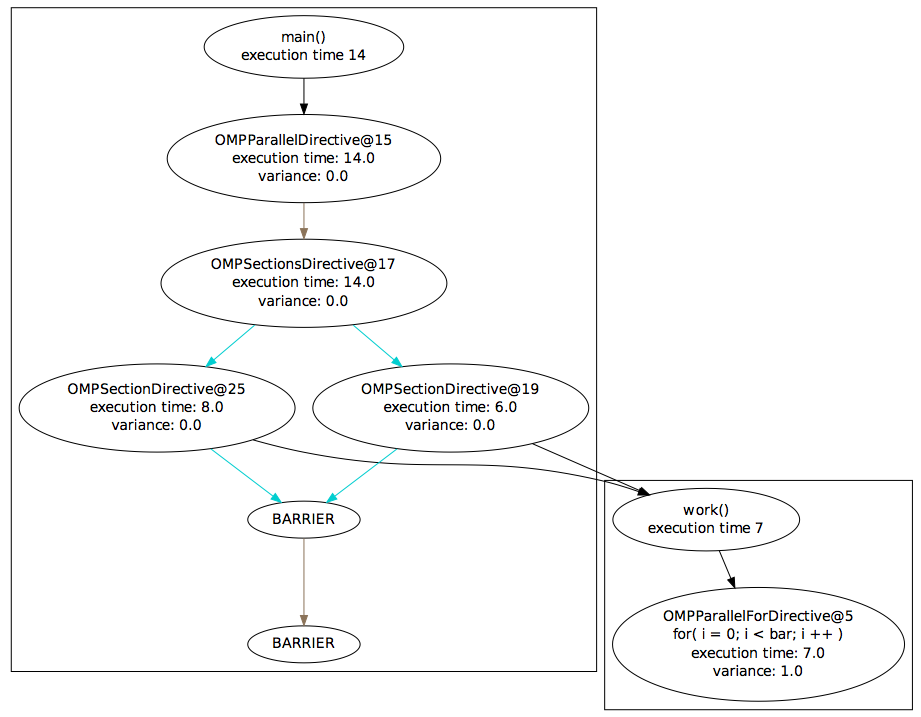
\includegraphics[width = 130mm, height = 76mm]{call_graph.png}
\caption{call graph example}
\label{call_graph}
\end{figure}


\section{Intrumentation for profiling}
\section{Profiling}

The priviously instrumented code is first executed $N$ times, which is given as input parameter, using as arguments the data contained in a specific text file. At each iteration the algorithm produces, for each function and pragma, their execution time and, in case of a $\#$pragma omp for or $\#$pragma omp parallel for, also the number of executed cycles. This data is gathered during the $N$ iterations and then the mean value of the execution time, executed loops and variance for each node is produced and saved in a log file code:\ref{log}. 

\lstset{language=XML}
\begin{lstlisting}[caption=Example log file, label=log]
<Log_file>
  <Hardware>
    <NumberofCores>4</NumberofCores>
    <MemorySize>2000</MemorySize>
  </Hardware>
  <Function>
    <FunctionLine>3</FunctionLine>
    <Time>7.0</Time>
    <Variance>1.0</Variance>
    <CallerId>[19, 25]</CallerId>
    <ChildrenTime>7.0</ChildrenTime>
  </Function>
...
  <Pragma>
    <FunctionLine>12</FunctionLine>
    <PragmaLine>25</PragmaLine>
    <Time>8.0</Time>
    <Variance>0.0</Variance>
    <Loops>-6.0</Loops>
    <CallerId>['17']</CallerId>
    <ChildrenTime>8.0</ChildrenTime>
  </Pragma>
  <Pragma>
    <FunctionLine>12</FunctionLine>
    <PragmaLine>19</PragmaLine>
    <Time>6.0</Time>
    <Variance>0.0</Variance>
    <Loops>8.0</Loops>
    <CallerId>['17']</CallerId>
    <ChildrenTime>6.0</ChildrenTime>
  </Pragma>
...
\end{lstlisting}

The new data is added to the flow graph previously produced to be used later in the scheduling algorithm. This graph is then saved as \emph{XML} file by saving nodes and edged separately, giving each a unique identifier code:\ref{complete_graph}.


\lstset{language=XML}
\begin{lstlisting}[caption=Enhanced graph, label=complete_graph]
<File>
  <Name>omp_test.cpp</Name>
  <GraphType>flow</GraphType>
  <Function id="30">
    <Name>work</Name>
    <ReturnType>int</ReturnType>
    <Parameters>
      <Parameter>
        <Type>int</Type>
        <Name>bar</Name>
      </Parameter>
    </Parameters>
    <Line>3</Line>
    <Time>7.0</Time>
    <Variance>1.0</Variance>
    <Callerids>
      <Callerid>19</Callerid>
      <Callerid>25</Callerid>
    </Callerids>
    <Nodes>
      <Pragma id="58">
        <Name>OMPParallelForDirective</Name>
        <Position>
          <StartLine>5</StartLine>
          <EndLine>8</EndLine>
        </Position>
        <Callerids>
          <Callerid>3</Callerid>
        </Callerids>
        <Time>7.0</Time>
        <Variance>1.0</Variance>
      </Pragma>
    </Nodes>
    <Edges>
      <Edge>
        <Source>30</Source>
        <Dest>58</Dest>
      </Edge>
    </Edges>
  </Function>
\end{lstlisting}


\section{Schedule generation}

The problem of finding the best possible schedule on a multicore architecture is known to be a \emph{NP} hard problem. Given $N$ tasks and $M$ computing cores, the problem consists of creating $K$, possibly lower than $M$, execution flows in order to assign each task to a single flow. Each flow represents a computing core onto which the task should be run. To find a good solution a recursive algorithm has been developed which, by taking advantage of a search tree fig:\ref{search_tree}, tries explore all possible solutions, pruning "bad" brenches as soon as possible. Often the algorithm could not finish in a reasonable time due to the big number of possible solutions; to solve this problem a timer has been added to stop the computation after a certain amount of time given as input. 

\begin{figure}[H]
\centering
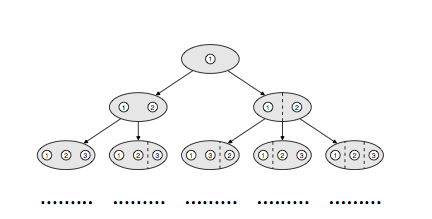
\includegraphics[width = 130mm, height = 76mm]{search_tree.png}
\caption{search tree}
\label{search_tree}
\end{figure}

At each level of the search tree a single task is considered; the algorithm inserts the task in each possible flow, checks if the partial solution is feasible and, if affermative, continues until all tasks have been set arriving to a leaf. To check if the partial solution is feasible the algorithm calculates the cost of the actual solution and compares it with the best solution found so far, then it checks that the number of created flows is less than a predefined number and that the timer has not expired; if all this requirements are met, the brench continues its execution, otherwise it is pruned. After that all task are set, if the requirements are fullfilled, the actual solution is compared with the optimal found so far and, in case, the actual one will become the new optimal solution. To calculate if a solution is better than another a simple heuristic has been used: the cost of a task is it's computation time, each flow has as cost the summation of all the costs of the containing tasks and the cost of a set of flows (solution or partial solution) is the maximum of the costs of the flows. Given this metric a solution is better than another if it has a lower cost. Having a low flow cost means that the flows are well balanced; it is also important to notice that the algorithm is working in a \emph{}breadth-first manner so that the number of flows is conservative, meaning that the lowest possible number is used to find the best solution. It is possible to easily add any number of pruning and cost metrics to improve the actual search algorithm

There is a small variation of the algorithm when a task containing a \emph{$\#$pragma parallel for} or \emph{$\#$pragma  for} is encountered. In this case the algorithm tryes to split the for loop as much as possible creating new tasks which are added to the task list. First the task is divided in two tasks and they are added to the task list, then the task is splitted in three checking this solution and so on until arriving to the number of available cores. The execution time of each task will be updated accordingly to the number of sub tasks in which it was splitted. 

A parallel version of this algorithm has also been developed in order to check more solutions in the same time. It is important to remember that in \emph{Python}, even if more threads are created, there is only a single interpreter, so all the threads execution is serialized; to avoid this problem the tool creates different processes, each with its own \emph{Python} interpreter. Given that the algorithm requires a lot of shared and private data which is updated at each computation step, the parallelisation of the algorithm would have been extremely complex, so an easier approach has been used. The same sequential algorithm is executed in parallel using for each process a randomized input order of the tasks. In this way each execution will produce all possible solutions in a different order; in any case after a certain amount of time all the processes will find all possible solutions, but with a timing contrain it is very likely that  more solutions are checked, in the same time, then in the sequential version. The algorithm terminates returning an optimal solution in the sequantial case and $K$ solutions in the parallel version; in this case the solutions are then compared and the best one is choosen as scheduling sequence. \\
It is important to notice that such a sequence could in principle not be schedulable, since the algorithm does not take care of precedence relations, but tries only to find the cheapest possible allocation. To check if the solution is feasible a second algorithm has been implemented following a modified version of the the parallel Chetto$\&$Chetto algorithm \cite{bbw2}.

This algorithm works in two phases, the first one sets the deadline for each task, while the second one sets its arrival time. To set the deadline, the algorithm sets the deadline of all the task with no predecessors to the expected deadline; then recursivly it sets the deadline of all task wich have all their successors deadline set by calculating the minimum of the difference between the computation time of the successor and the deadline of the successor. 

In the second phase the algorithm sets all the arrival times of task with no predecessors to zero; after that it recursivly sets the arrival time of all tasks, which have the arrival time of all predecessors set, by calculating the maximum between all the arrival time of the predecessors, belonging to the same flow, and the deadline of all the tasks which are assigned to a different flow. This is due to the following fact: \\
let $\tau_j$ be a predecessor of $\tau_i$, written as $\tau_j \rightarrow \tau_i$, with arrival time $a_i$ and let $F_k$ be the flow $\tau_i$ belongs to. If $\tau_j \in F_k$, then the precedence relation is already enforced by the previously assigned deadlines. So it is sufficient to ensure that task $\tau_i$ is not activated before $\tau_j$. This can be achived by ensuring that :
\begin{center}$ a_i \ge  {a_i}^{prec} = \smash{\displaystyle\max_{\tau_j \rightarrow \tau_i,\tau_j \in F_k} }\{a_j$\}.\end{center}
If $\tau_j \notin F_k$, we cannot assume that $\tau_j$ will be allocated on the same physical core as $\tau_i$, thus we do not know its precise finishing time. Hence, $\tau_i$ cannot be activated before $\tau_j$'s deadline $d_j$, that is:
\begin{center}$ a_i \ge  {d_i}^{prec} = \smash{\displaystyle\max_{\tau_j \rightarrow \tau_i,\tau_j \notin F_k} }\{d_j$\}.\end{center}
The algorithm checks then that all the deadlines and arrival times are consistent and in case produces the scheduling schema.

\section{Instrumentation for the execution}
\section{Run-time support}

\chapter{Implementation}
\section{Scheduling XML schema}
\section{Instrumentation for Profiling}
\section{Profiling implementation}
\section{Schedule generating tool}
\section{Instrumentation for the execution}
\section{Run-time support}

\chapter{Performance evaluation}
\section{A computer vision application}
\section{Results with statistics}

\chapter{Conclusions}
\section{Achieved results}
\section{Future development}

\begin{thebibliography}{9}
\bibitem{bbw} Giorgio Buttazzo, Enrico Bini, Yifan Wu. \emph{Partitioning parallel applications on multiprocessor reservations}. Scuola Superiore Sant’Anna, Pisa, Italy
\bibitem{bbw2} Giorgio Buttazzo, Enrico Bini, Yifan Wu. \emph{Partitioning real-time applications over multi-core reservations}. Scuola Superiore Sant’Anna, Pisa, Italy
\bibitem{mfp} Ricardo Garibay-Martinez, Luis Lino Ferreira and Luis Miguel Pinho, \emph{A Framework for the Development of Parallel and Distributed Real-Time Embedded Systems}
\bibitem{pop}Antoniu Pop (1998). \emph{OpenMP and Work-Streaming Compilation in GCC}. 3 April 2011, Chamonix, France

\end{thebibliography}

\end{document}